\documentclass{beamer}
\usetheme{Boadilla}
\usecolortheme{beaver}
%\usepackage{graphicx}
%\usepackage{minted}
%\usepackage[numbers]{natbib}
%\usepackage{float}
%\usepackage{multicol}
%\usepackage[magyar]{babel}
\usepackage{hyperref}
\usepackage{multimedia}
%\usepackage{comment}
%\usepackage{ragged2e}

\hypersetup{colorlinks=true, linkcolor=blue, filecolor=magenta, urlcolor=cyan}
\urlstyle{same}

\title{Járművek trajektóriáinak előrejelzése machine learning modellekkel}
\author{Péter Bence Mérnökinformatika BSc 6. félév}%\\Mérnökinformatika BSc 6. félév\\Konzulensek:\\Dr. Horváth András egyetemi docens\\Agg Áron PhD hallgató}
\institute{Széchenyi István University}

\begin{document}

\begin{frame}
\titlepage
\end{frame}

\begin{frame}
\frametitle{Tartalom}
\tableofcontents
\end{frame}

\section{Bevezetés}
\begin{frame}{Bevezetés}
\centering
%\includegraphics[scale=0.3]{deepsort_yolo_figs/gépilátás_modified.jpg}
\movie[showcontrols=true]{\includegraphics[scale=0.3]{../deepsort_yolo_figs/gépilátás_modified.jpg}}{demo_bevezetes.mp4}
\end{frame}


\section{Objektumdetektálás}
\begin{frame}{Objektumdetektálás}
    \begin{figure}
        
\includegraphics[scale=0.07]{yolo_logo.png}
    \end{figure}
    \begin{columns}
        \column{0.5\textwidth} 
        \centering
        \begin{figure}
            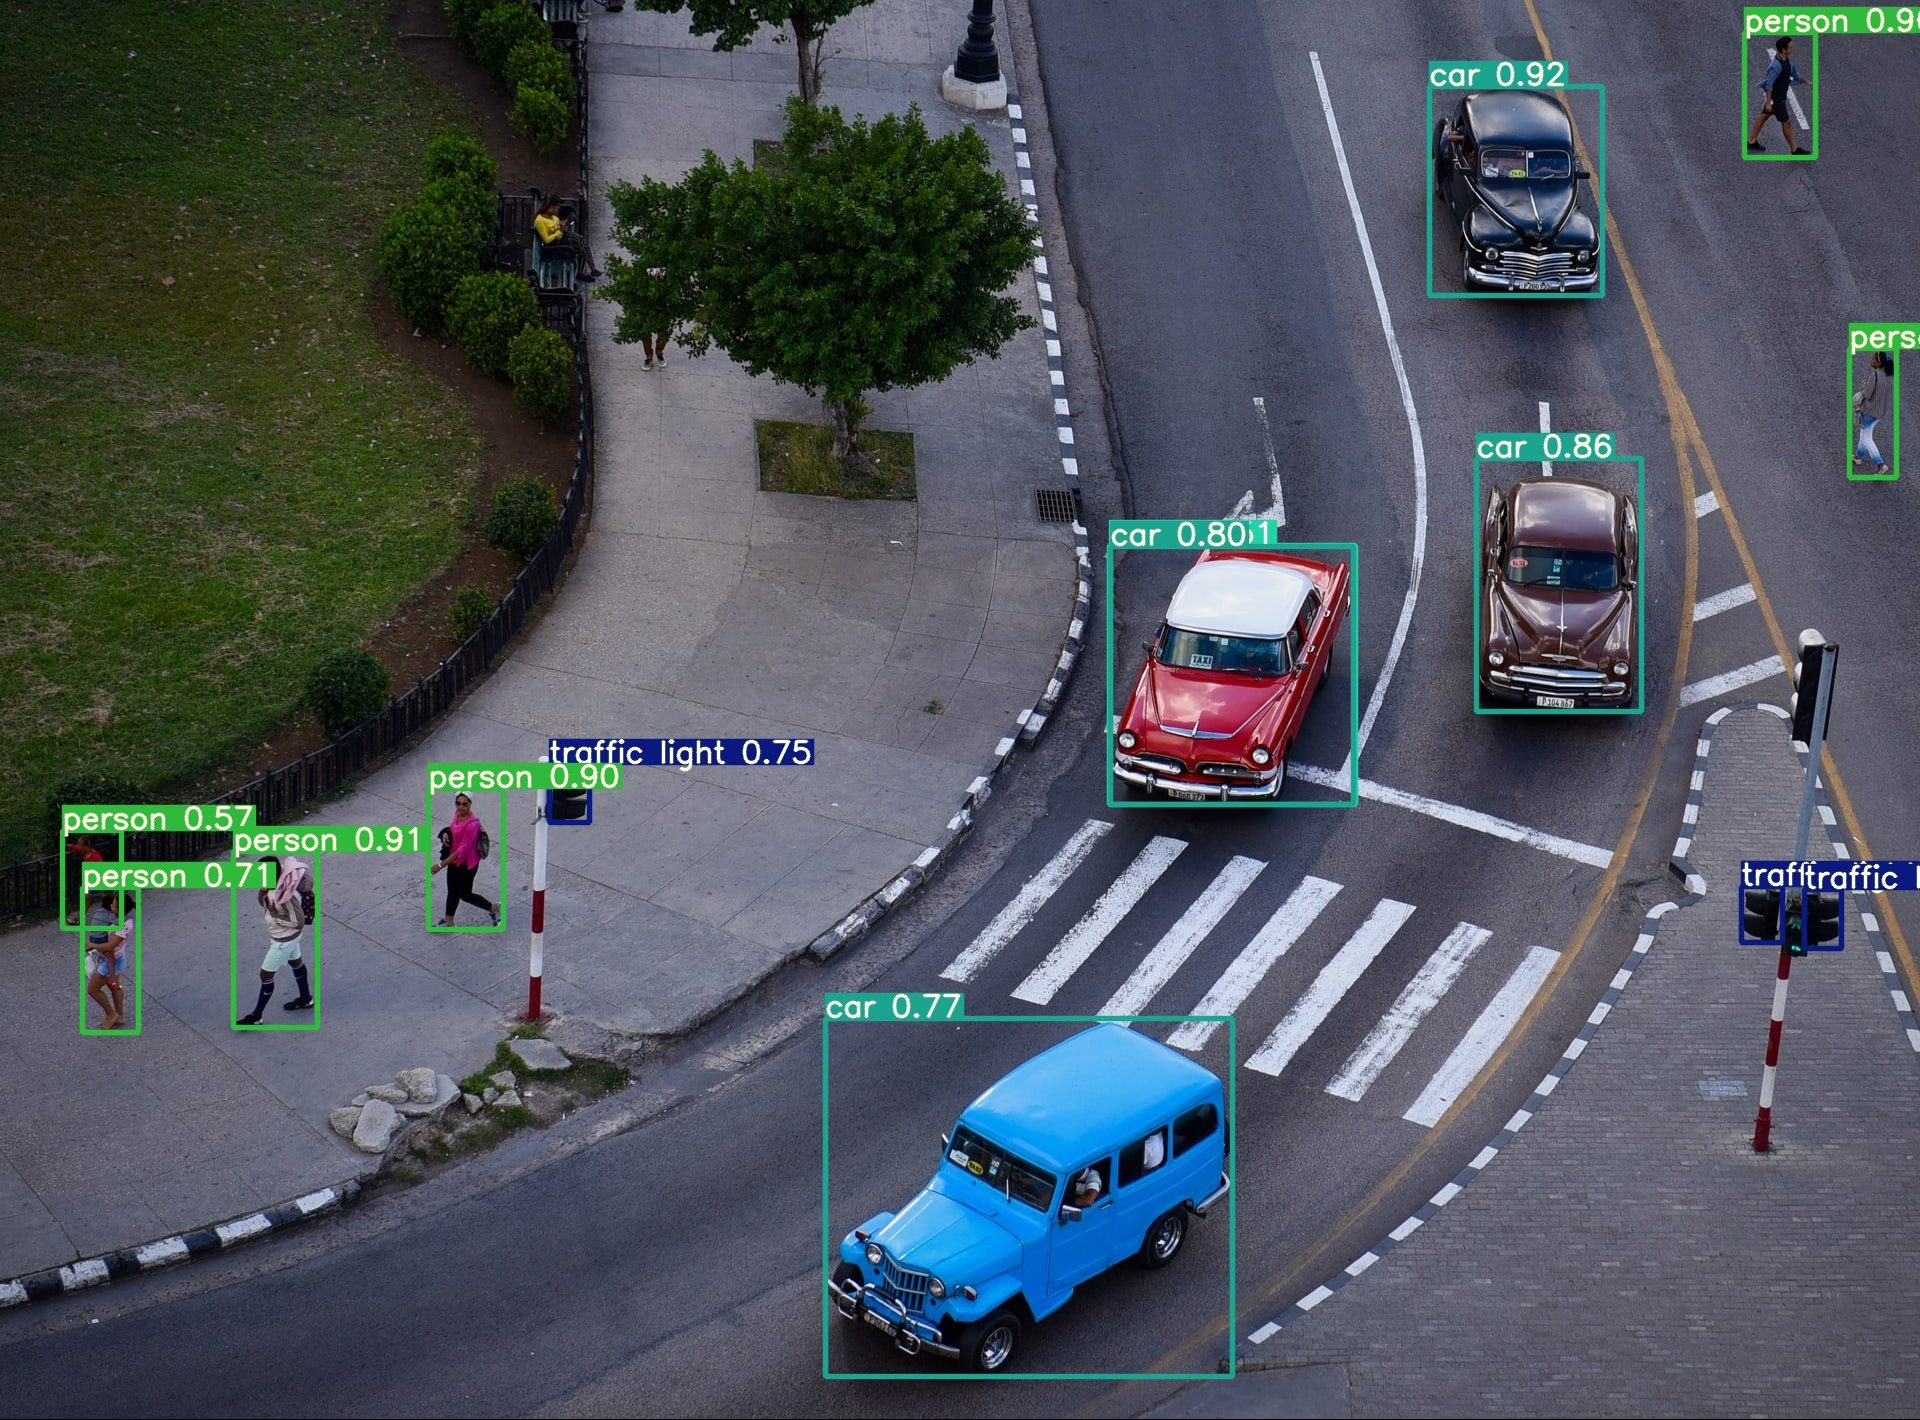
\includegraphics[scale=0.1]{yolo_img.jpg} 
        \end{figure}

        \column{0.5\textwidth}
        \centering
        \begin{figure}
            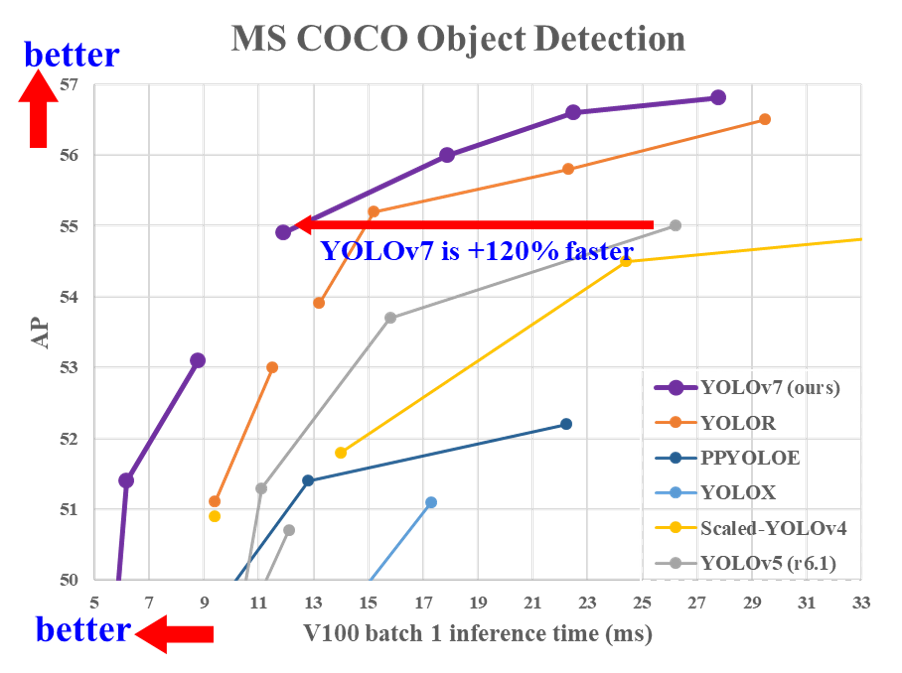
\includegraphics[scale=0.35]{../performance.png}
        \end{figure}
    \end{columns}
\end{frame}

\section{Objektumkövetés}
\begin{frame}{Objektumkövetés}
    \centering
    \begin{figure}
        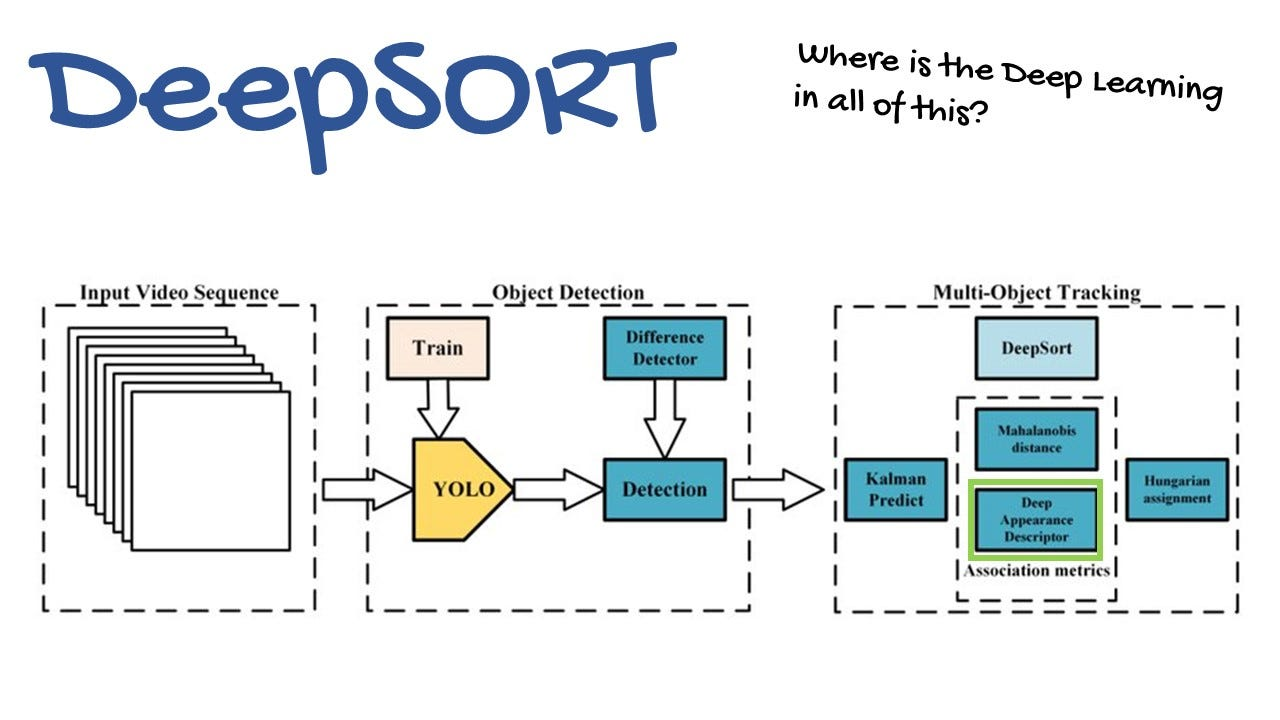
\includegraphics[scale=0.25]{deepsort_flowchart.jpg} 
    \end{figure}
\end{frame}

\section{Machine Learning}
\begin{frame}{Machine Learning}
    \centering
    \begin{figure}
        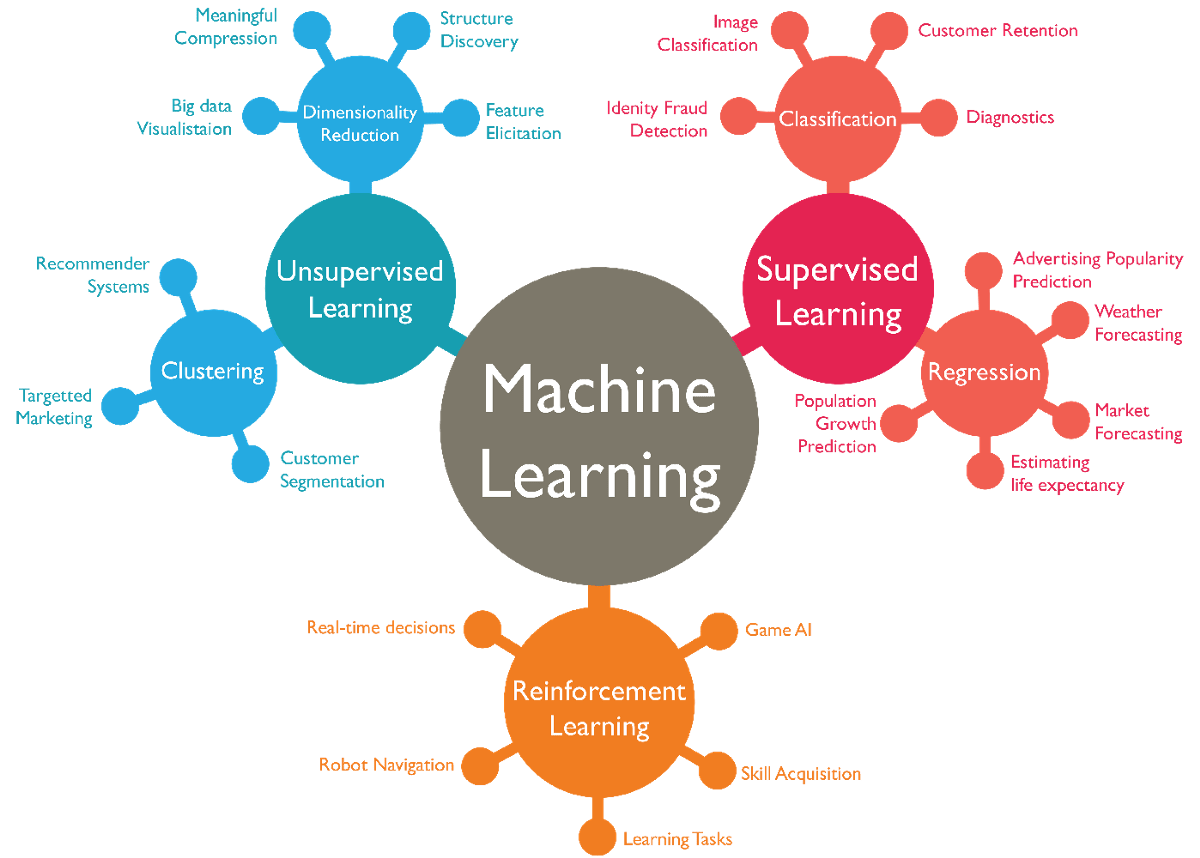
\includegraphics[scale=0.2]{machine_learning.png}    
    \end{figure}
\end{frame}
\subsection{Unsupervised learning}
\begin{frame}{Unsupervised learning}
    \begin{itemize}
        \item Nincsenek előre meghatározott osztályok
        \item Az algoritmus saját maga próbálja csoportokba rendezni a adatokat
    \end{itemize}
    \begin{figure}
        \includegraphics[scale=0.3]{unsupervised_learning.png}
    \end{figure}
\end{frame}
\subsection{Supervised learning}
\begin{frame}{Supervised learning}
    \begin{itemize}
        \item Előre meghatározott osztályok alapján
        \item Az algoritmust tanítani kell példa adatokkal 
        \item Amiket vagy kézzel, vagy klaszterezéssel rendezünk osztályokba
    \end{itemize}
    \begin{figure}
        \includegraphics[scale=0.25]{supervised_learning.jpeg}
    \end{figure}
\end{frame}

\section{Klaszterezés}
\begin{frame}{Klaszterezés}
    \begin{itemize}
        \item Bemeneti adatok: gyűjtött trajektóriák objektumdetektálás és követés segítségével
        \item Feature vektorok: trajektóriák be és kimeneti pontjai
    \end{itemize}
    \begin{figure}
        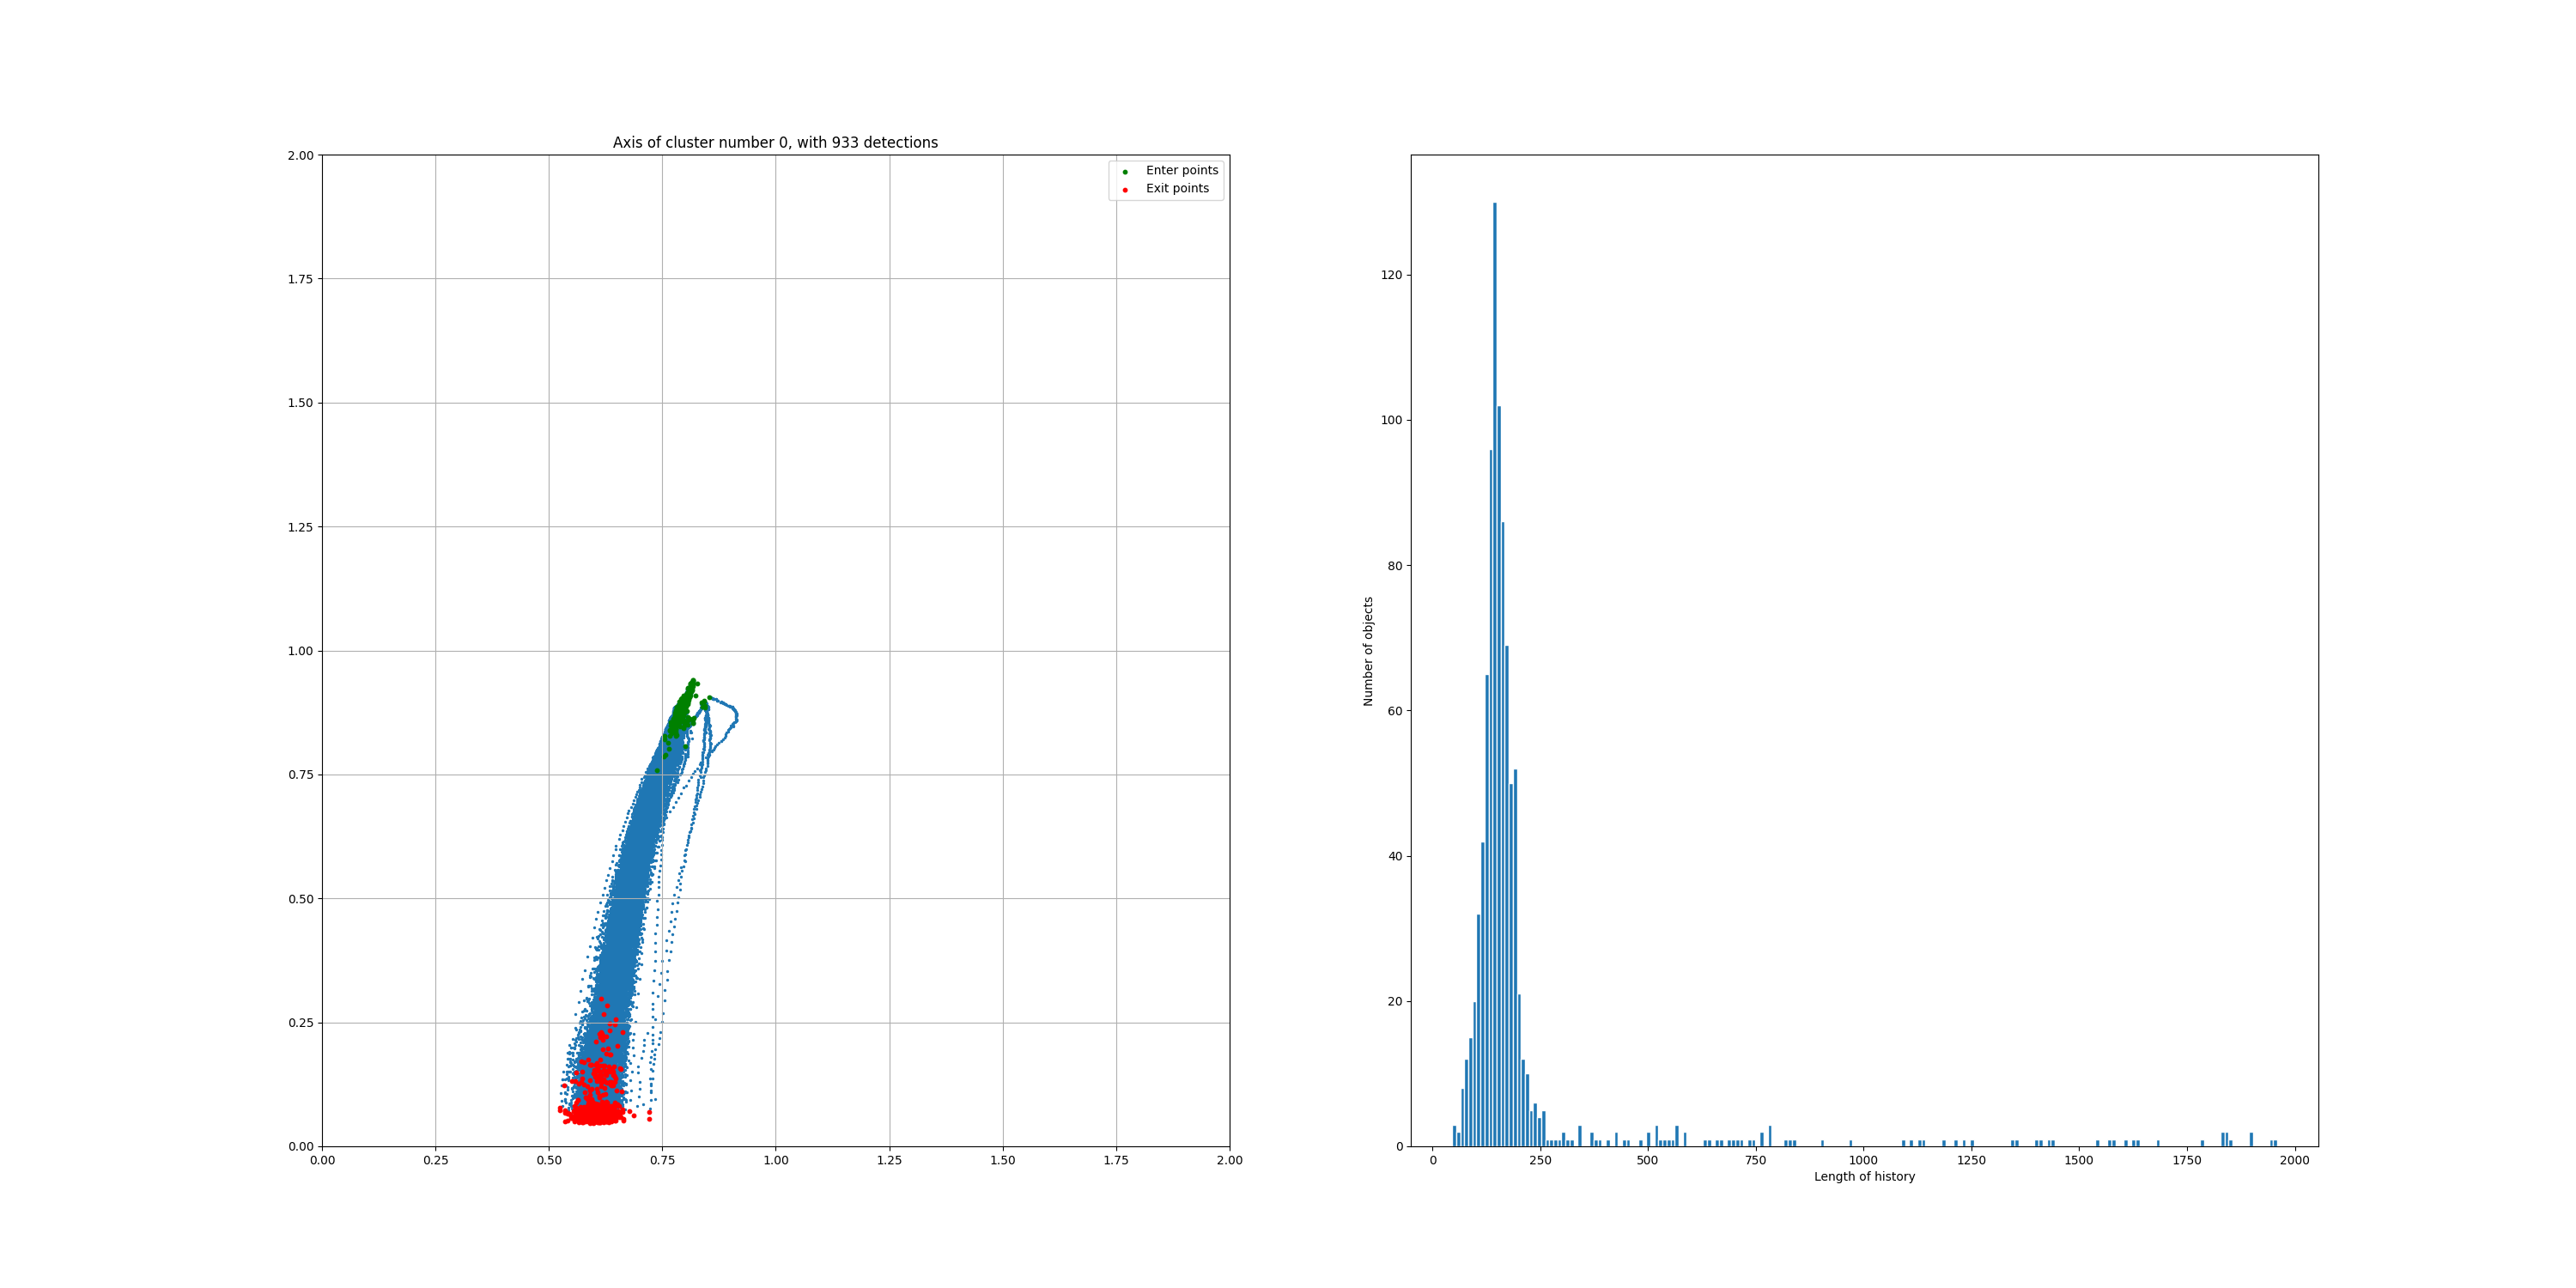
\includegraphics[scale=0.15]{../clustering/n_cluster_0_n_tracks_933.png}
    \end{figure}
\end{frame}

\subsection{Trajektória}
\begin{frame}{Trajektória}
   \begin{figure}
        \includegraphics[scale=0.15]{trajektoriak/car1_1.png}
        \includegraphics[scale=0.15]{trajektoriak/car1_2.png}
        \includegraphics[scale=0.15]{trajektoriak/car1_3.png}
        \includegraphics[scale=0.15]{trajektoriak/car1_4.png}
   \end{figure} 
   \begin{figure}
        \includegraphics[scale=0.2]{trajektoriak/car2_1.png}
        \includegraphics[scale=0.2]{trajektoriak/car2_2.png}
        \includegraphics[scale=0.2]{trajektoriak/car2_3.png}
        \includegraphics[scale=0.2]{trajektoriak/car2_4.png}
   \end{figure} 
\end{frame}

\subsection{Adatok tisztítása}
\begin{frame}{Adatok tisztítása}
    \begin{itemize}
        \item Több különböző zajforrás
        \begin{itemize}
            \item YOLO késői detektálás és követés (a járművet már csak akkor veszi észre amikor bennt van a kereszteződésben)
            \item YOLO fals detektálás (rendőrlámpát vagy táblát autónak néz)
            \item DeepSORT áttapadások (egymáshoz közel elhaladó járművek identitása felcserélődik)
        \end{itemize} 
        \item Megoldások
        \begin{itemize}
            \item Kép relatív széleinek megtalálása min-max kereséssel (az utakat nem biztos, hogy a kép szélétől széléig látjuk, hanem a kép közepétől kezdődve, ezt okozhatja egy nagy épület)
            \item Szűrés trajektóriák kezdő és végpontjainak euklideszi távolsága alapján
            \item Szűrés trajektóriák egymást követő detektálásai közötti távolságokkal
        \end{itemize} 
    \end{itemize}   
\end{frame}

\subsection{Zajos vs Szűrt}
\begin{frame}{Zajos vs Szűrt}
    \begin{figure}
        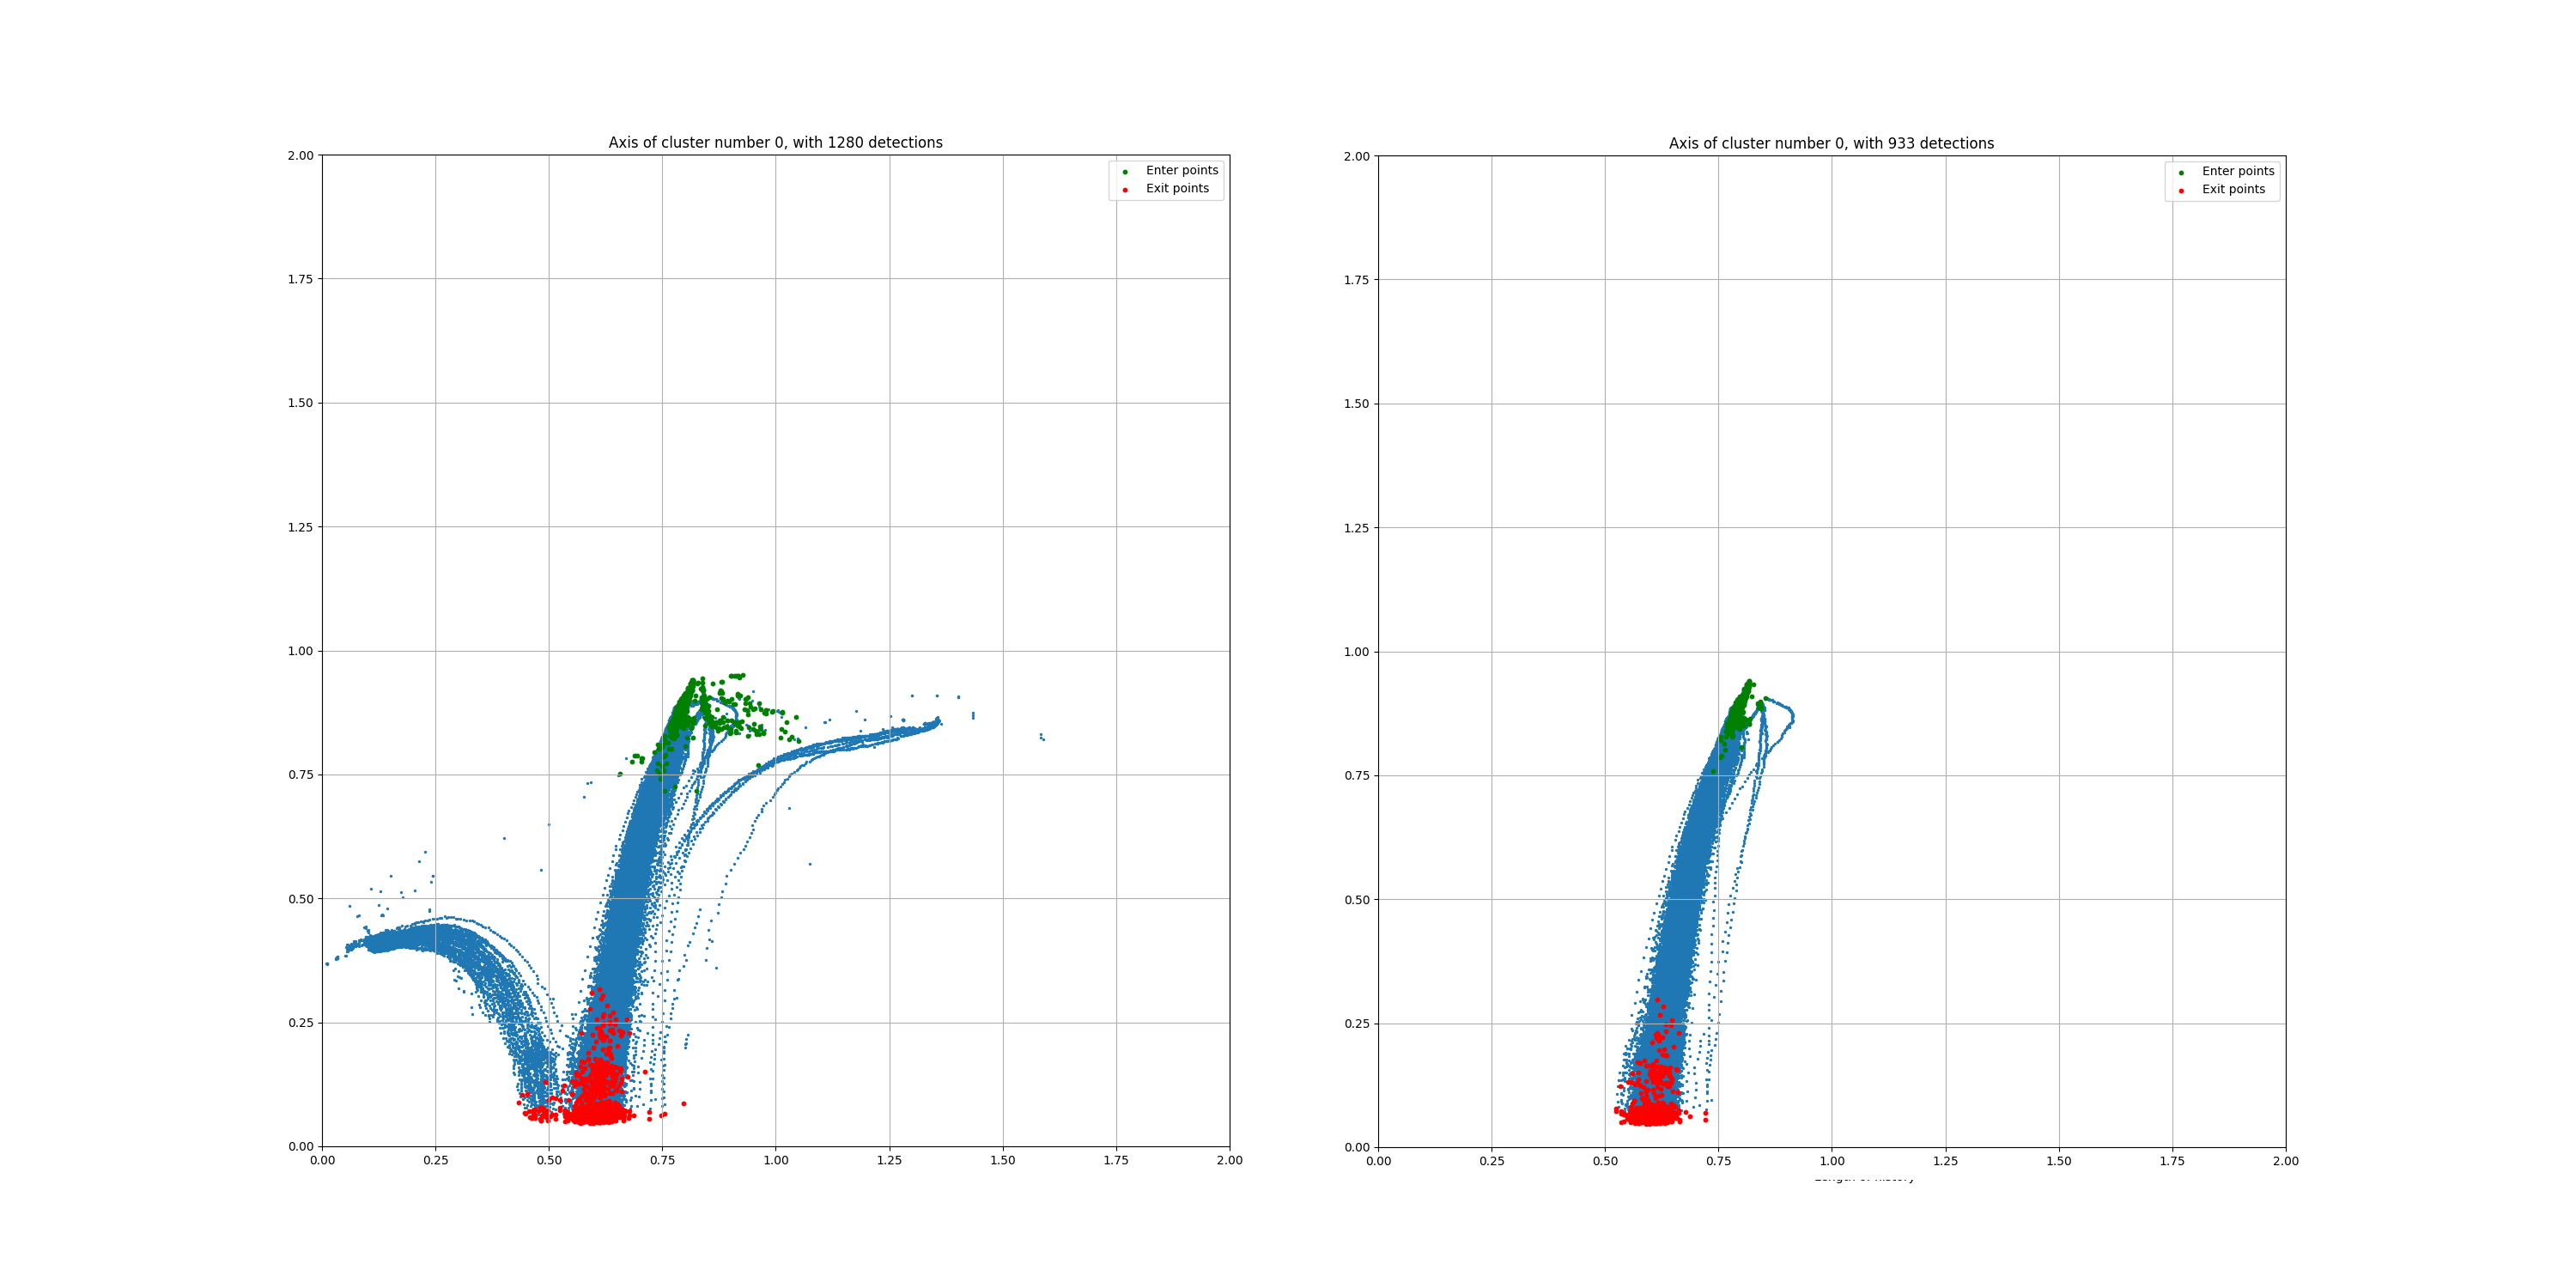
\includegraphics[scale=0.1]{../clustering/n_cluster_0_before_after.png}
        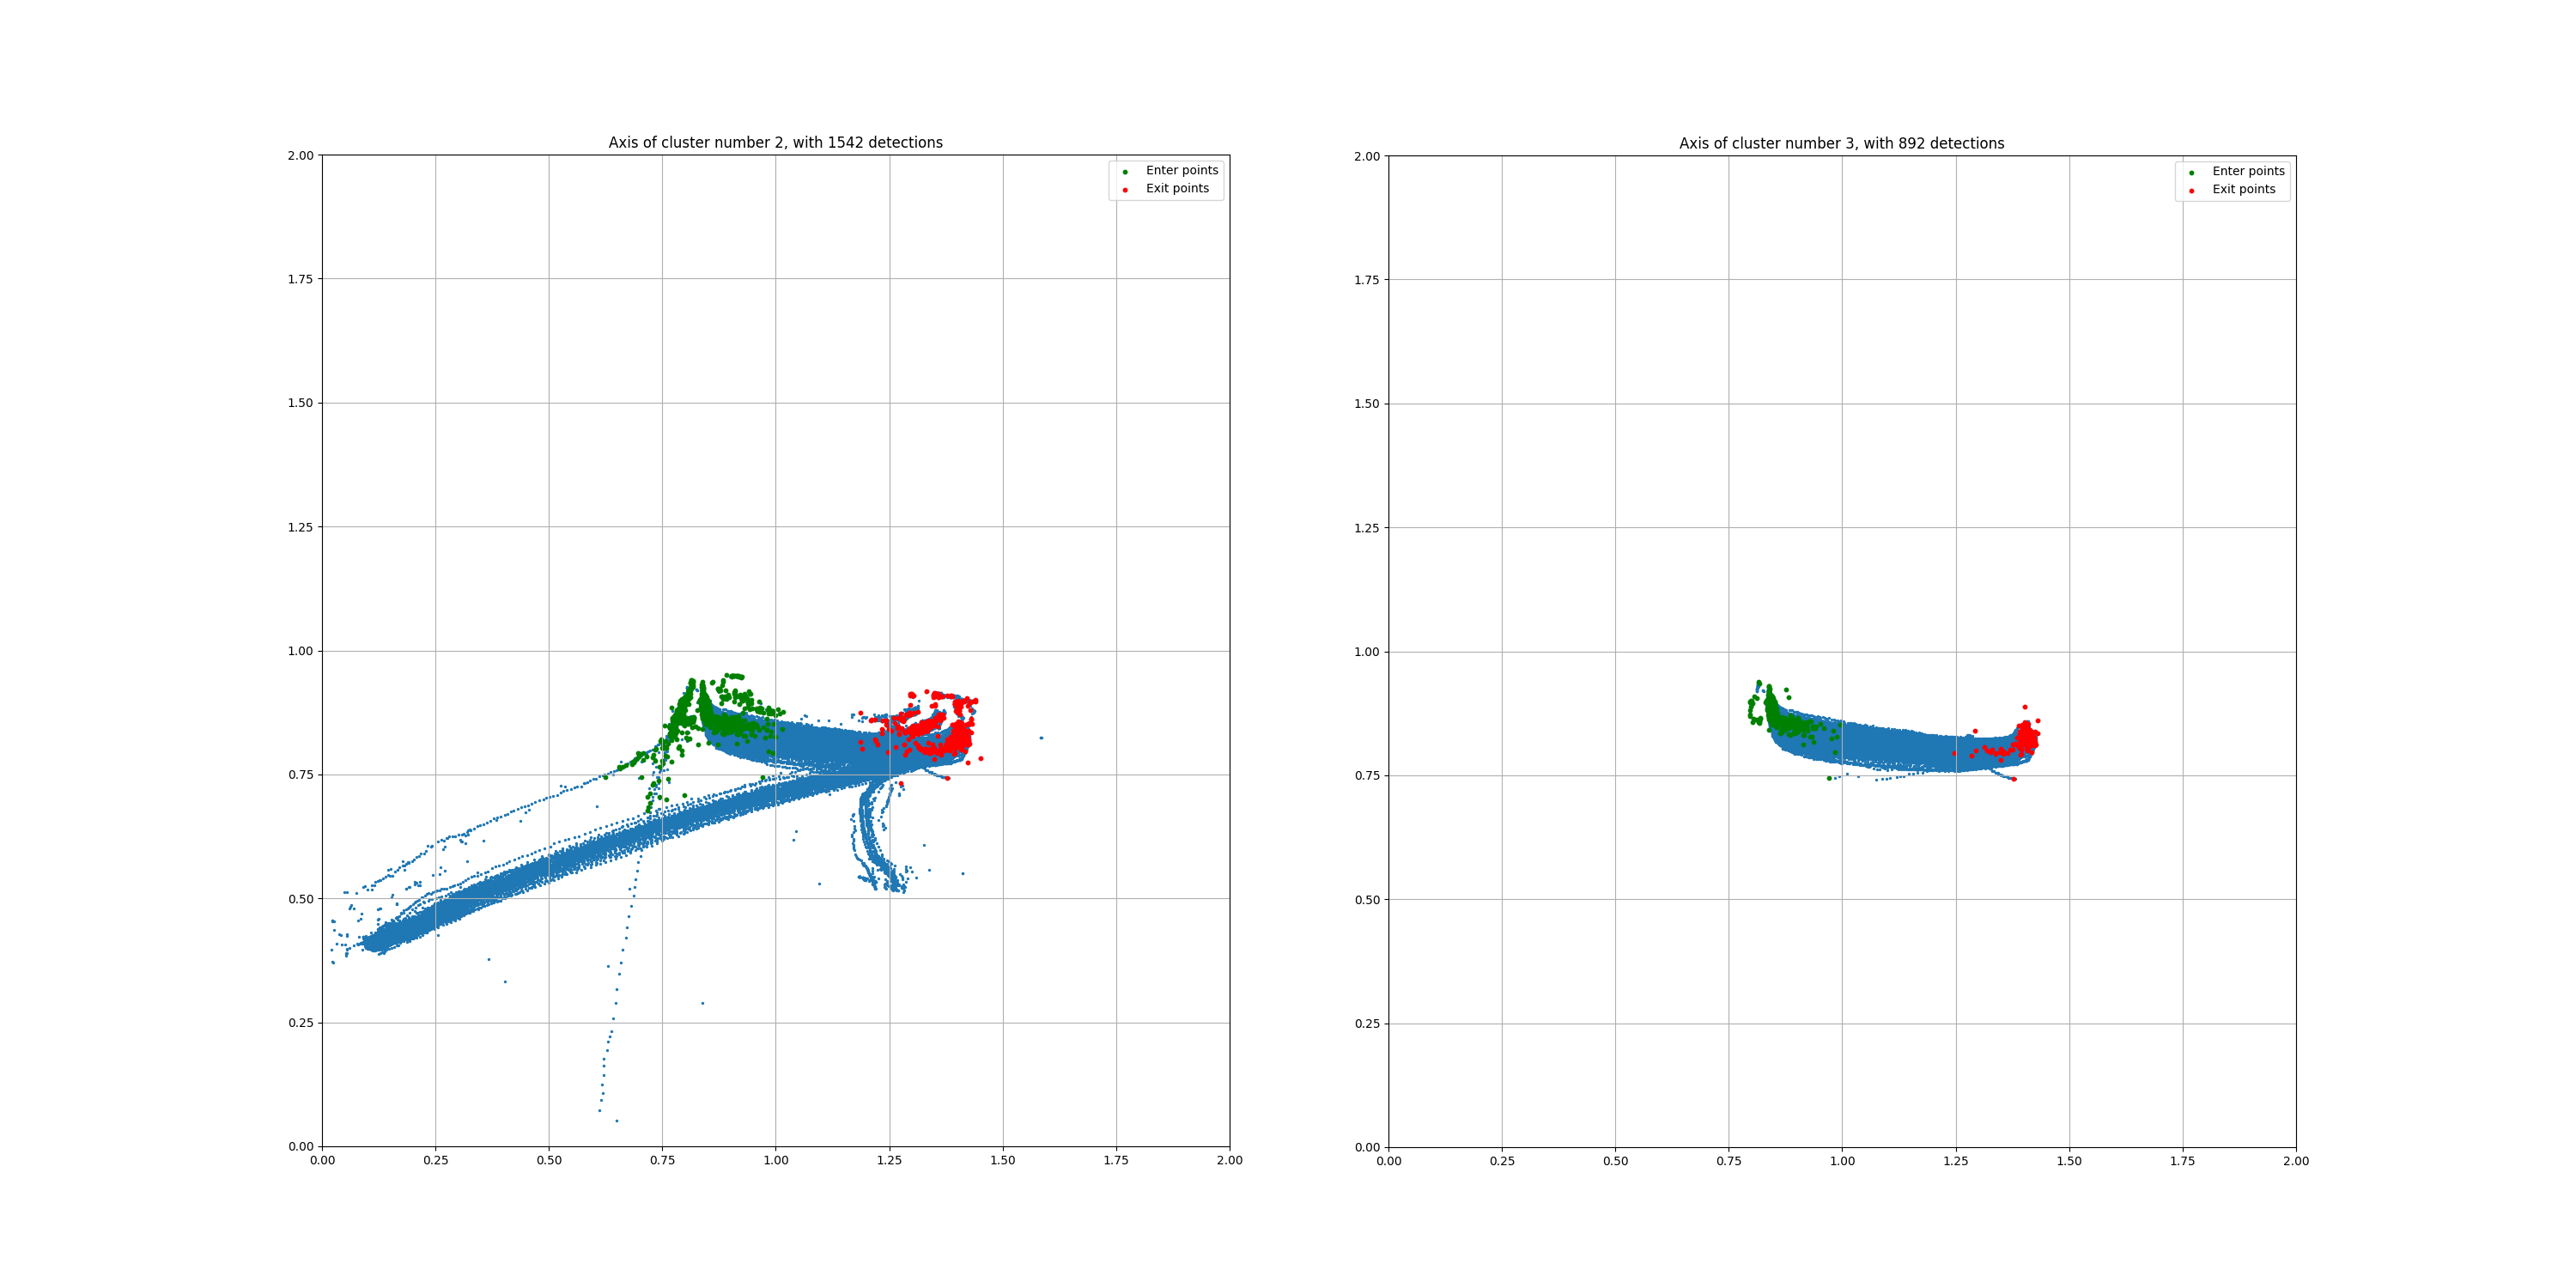
\includegraphics[scale=0.1]{../clustering/n_cluster_2_before_after.png}
    \end{figure}
\end{frame}

\subsection{OPTICS vs KMeans, BIRCH}
\begin{frame}{OPTICS vs KMeans, BIRCH}
    \begin{itemize}
        \item Klaszterezést több algoritmussal teszteltük
        \item KMeans, BIRCH, DBSCAN, OPTICS
        \item OPTICS adta a legjobb eredményeket
    \end{itemize}
    \begin{columns}
        \column{0.5\textwidth}
        \begin{figure}
            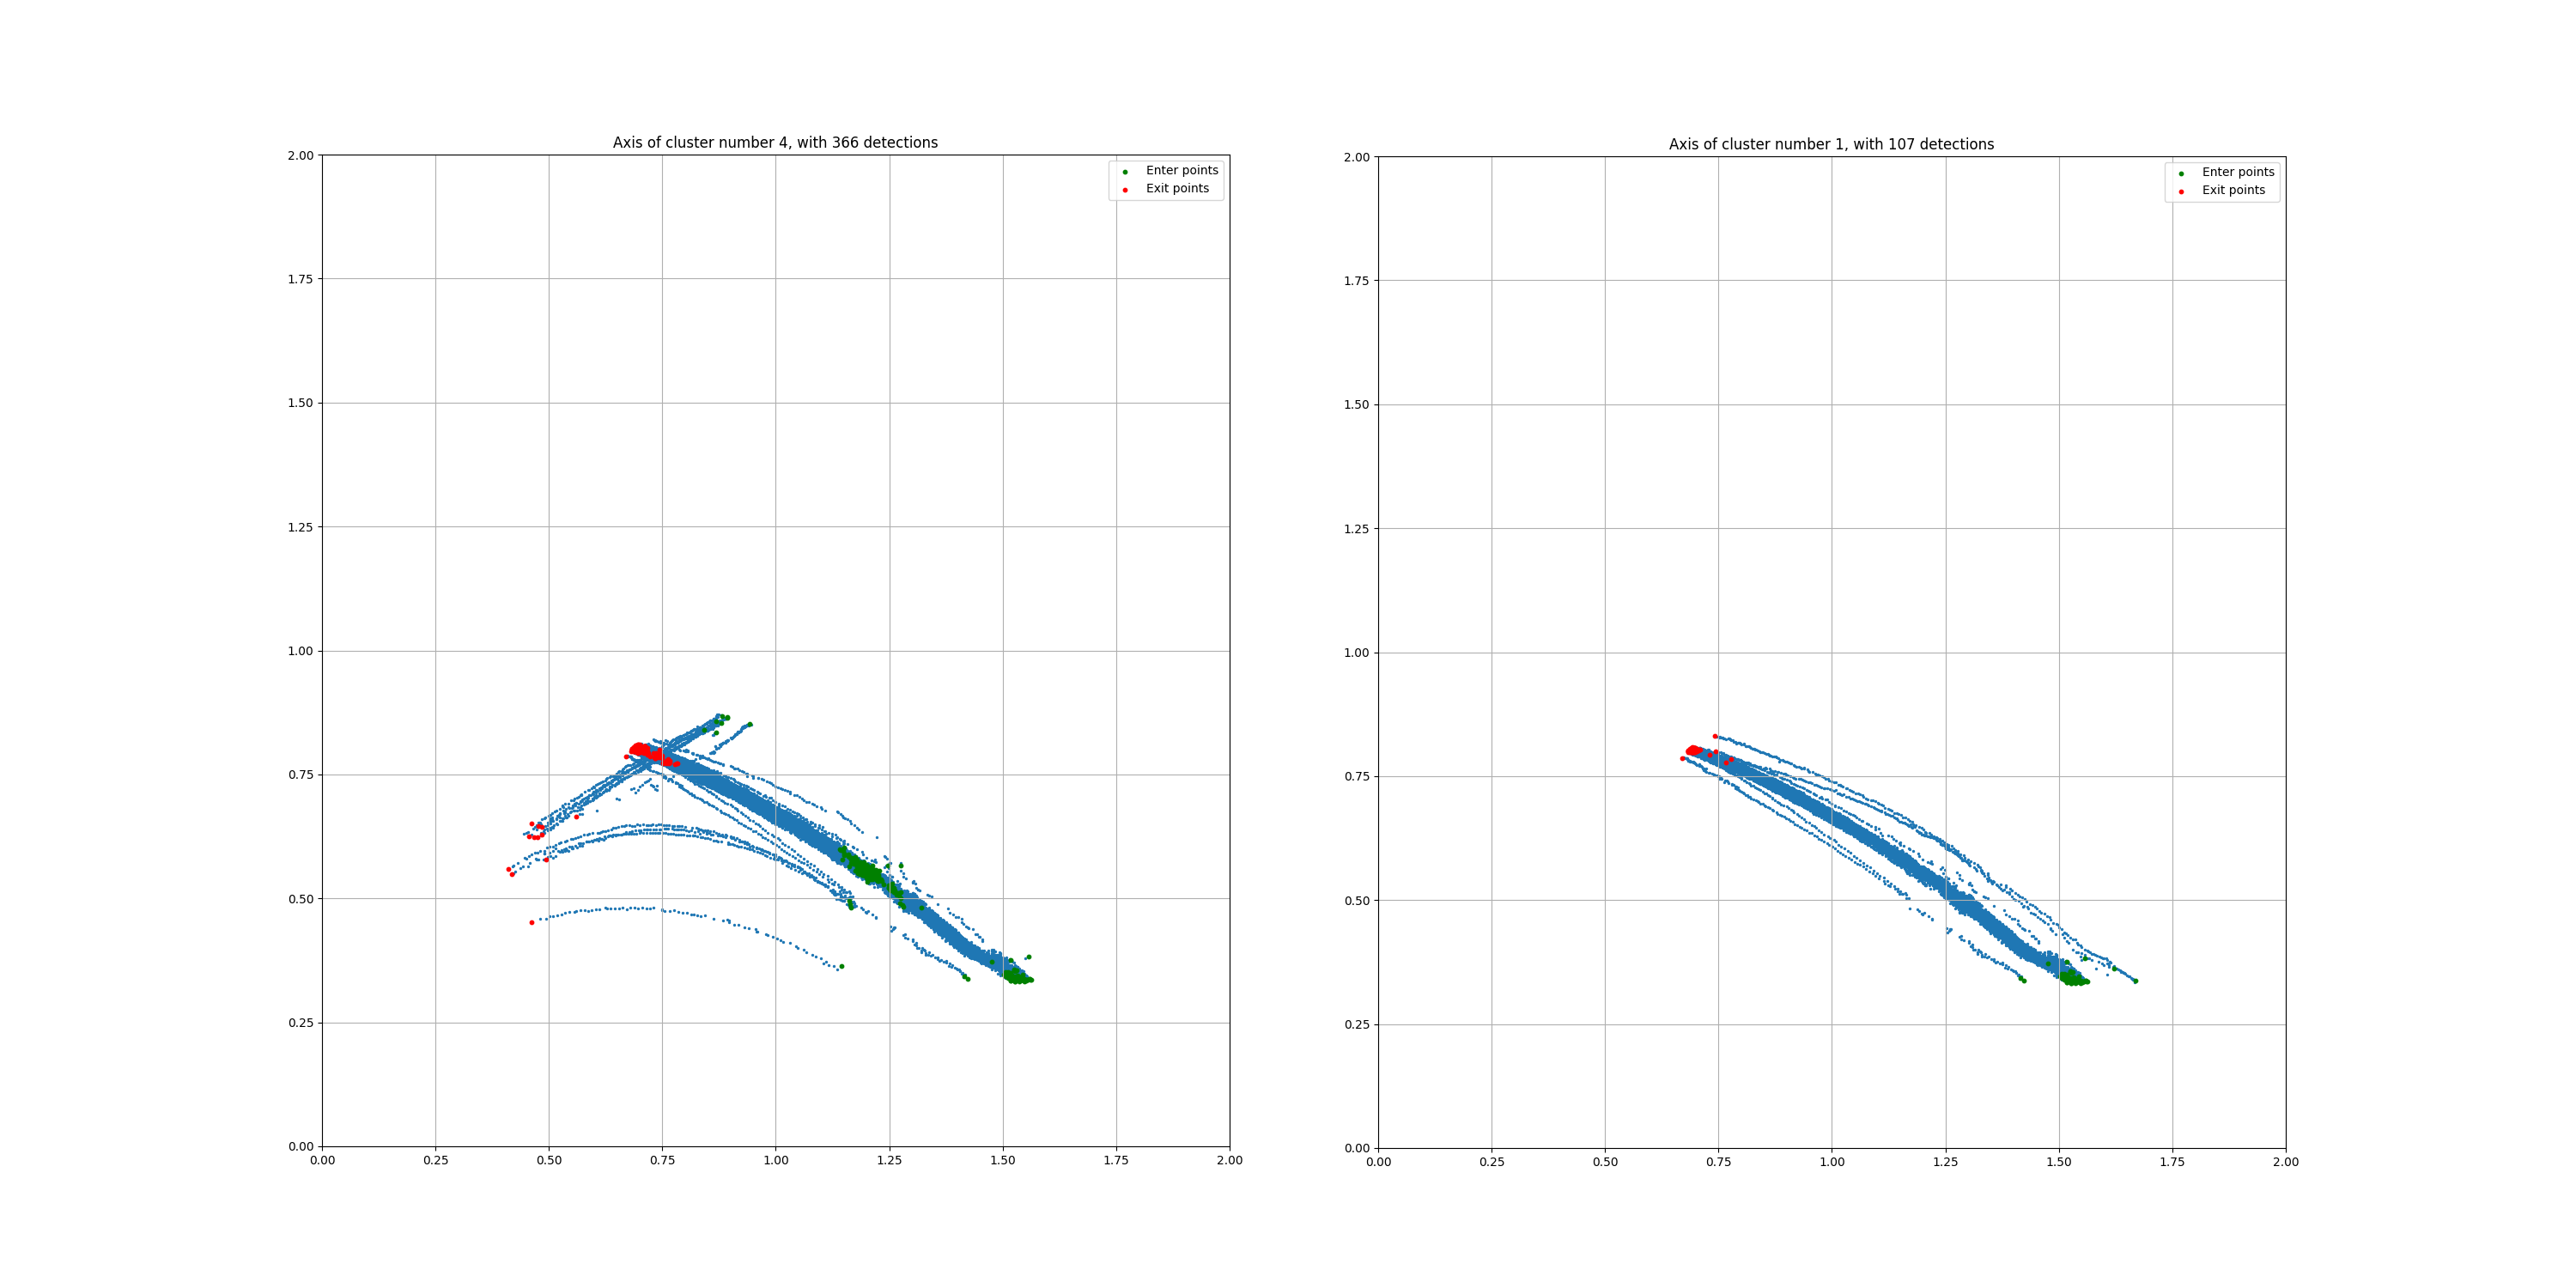
\includegraphics[scale=0.08]{../bad_clustering/example_kmeans_vs_optics.png}
        \end{figure}
        \column{0.5\textwidth}
        \begin{figure}
            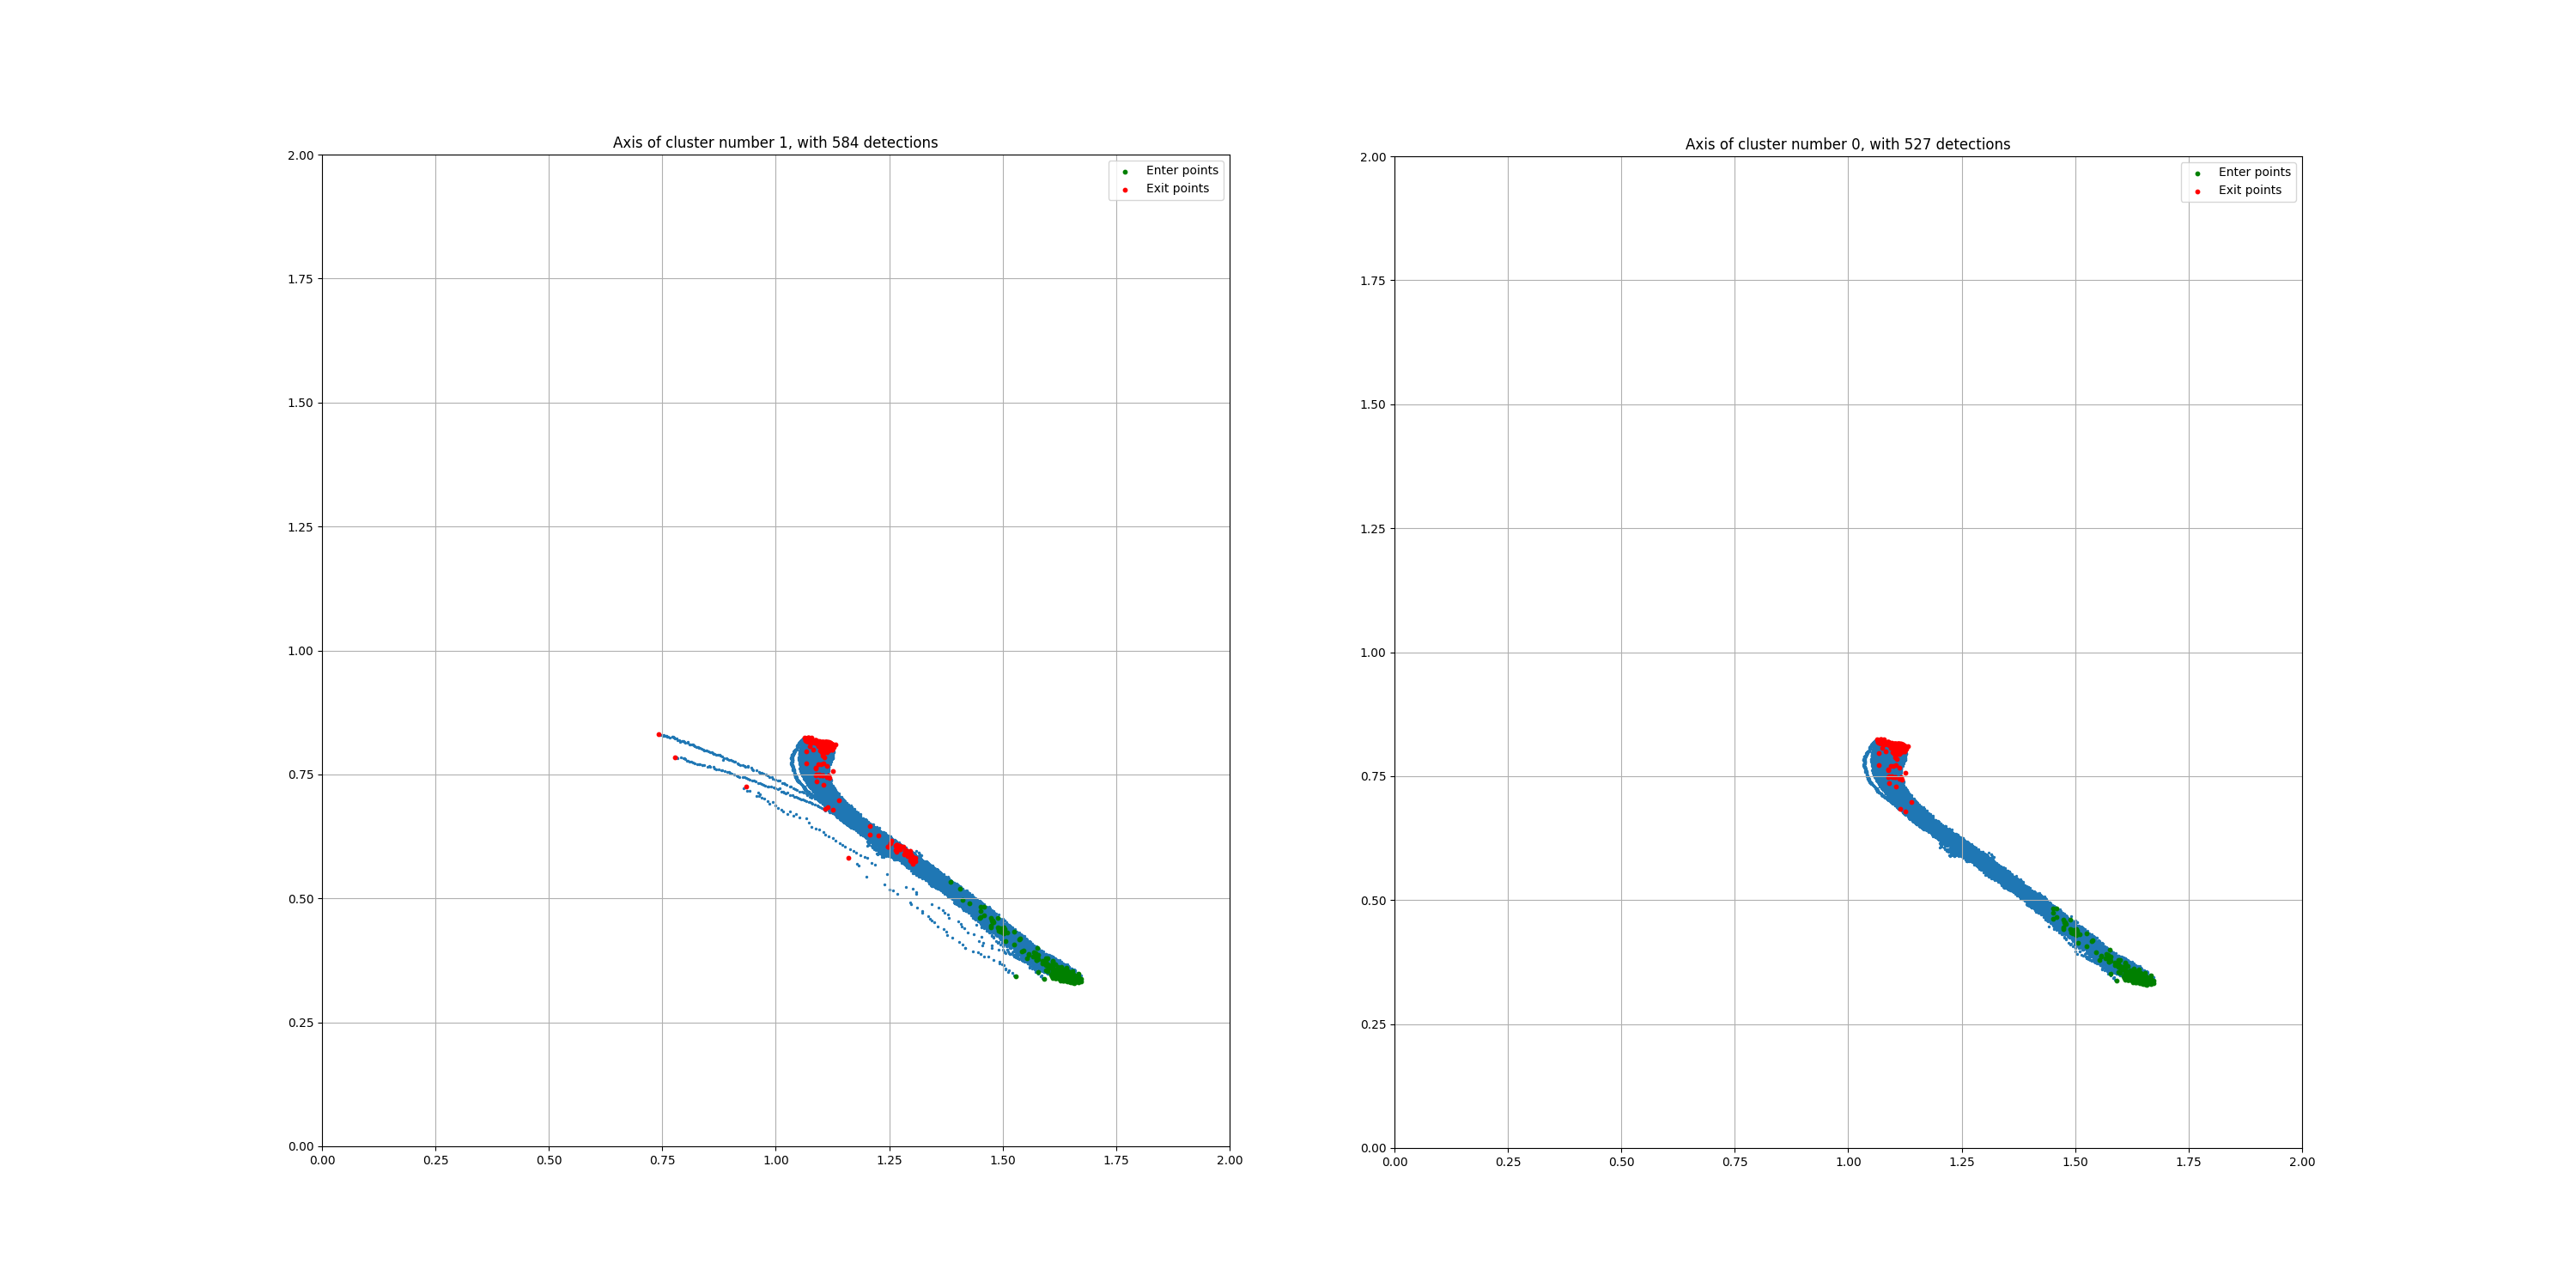
\includegraphics[scale=0.08]{../bad_clustering/example_birch_vs_optics.png}
        \end{figure}
    \end{columns}
\end{frame}

\subsection{OPTICS vs DBSCAN}
\begin{frame}{OPTICS vs DBSCAN}
    \centering
    \begin{figure}
        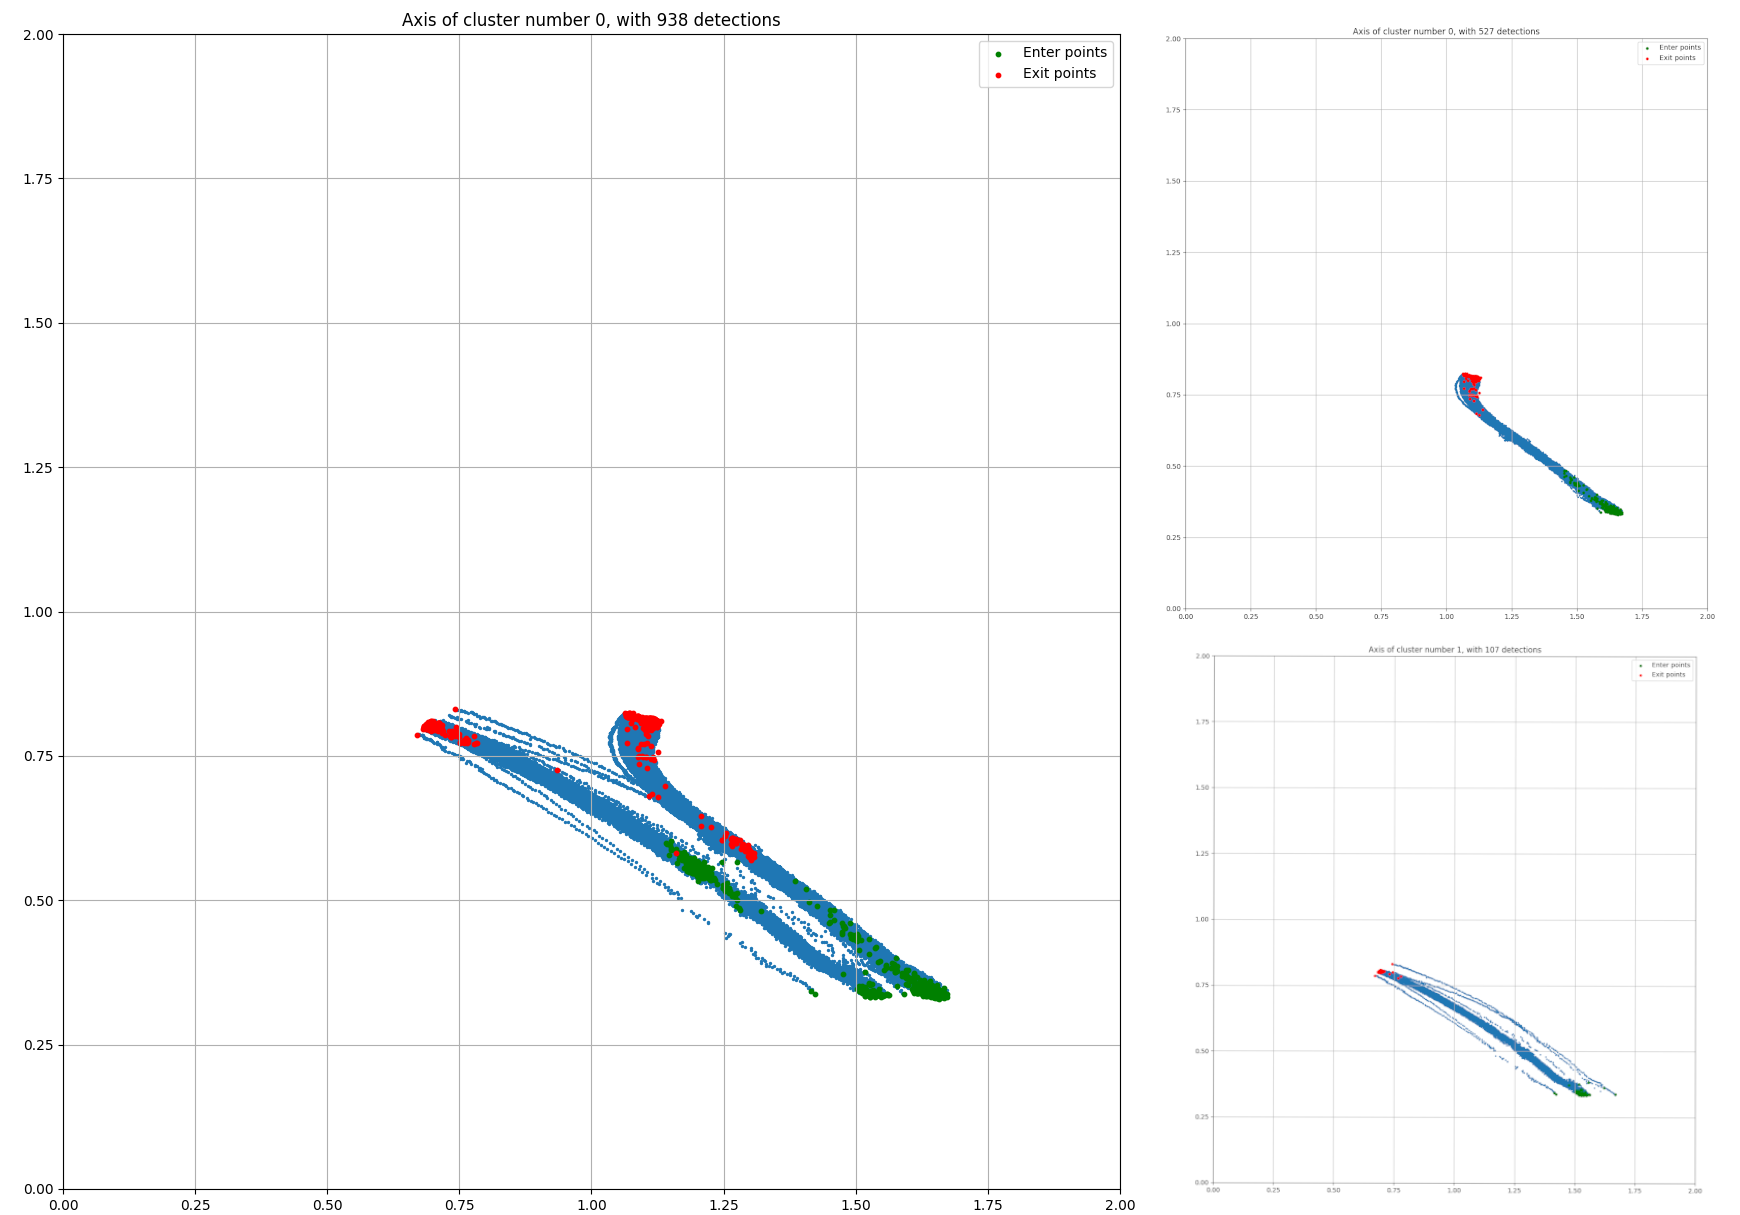
\includegraphics[scale=0.2]{../bad_clustering/example_dbscan_vs_optics_merged_cluster.png}
    \end{figure}
\end{frame}

\section{Klasszifikáció}
\begin{frame}{Klasszifikáció}
    \begin{itemize}
        \item Feature vektorok: trajektóriák felosztása több kisebb részre, amik a valós idejű futásból származó trajektóriákhoz hasonlít
        \begin{itemize}
            \item v1: trajektória kezdőkoordinátája, sebessége, középső koordinátája, utolsó koordinátája, sebessége 
            \item v7: trajektória kezdőkoordinátája $\cdot 1$, sebessége $\cdot 100$, utolsó koordinátája $\cdot 2$, sebessége $\cdot 200$
        \end{itemize}
        \item Adathalmaz dúsítása: mivel egy trajektóriából több feature vektort csináltunk, így a tanító adathalmazt is megnöveltük
    \end{itemize}
\end{frame}

\subsection{Klasszifikációs algoritmusok}
\begin{frame}{Klasszifikációs algoritmusok}
    \begin{itemize}   
        \item K-NearestNeighbors, SupportVectorMachine, DecisionTree 
    \end{itemize}
    \begin{table}[]
    \begin{tabular}{|lccc|}
    \hline
    \multicolumn{4}{|c|}{\begin{tabular}[c]{@{}c@{}}Average Accuracy Feature Vector v1\end{tabular}}    \\ \hline
    \hline
    \multicolumn{1}{|l|}{Metrics} & \multicolumn{1}{c|}{Balanced} & \multicolumn{1}{c|}{Top 1}   & Top 2   \\ \hline
    \multicolumn{1}{|l|}{KNN}     & \multicolumn{1}{c|}{94.16\%}  & \multicolumn{1}{c|}{96.71\%} & 99.46\% \\ \hline
    \multicolumn{1}{|l|}{SVM}     & \multicolumn{1}{c|}{81.65\%}  & \multicolumn{1}{c|}{90.82\%} & 98.05\% \\ \hline
    \multicolumn{1}{|l|}{DT}      & \multicolumn{1}{c|}{93.11\%}  & \multicolumn{1}{c|}{94.88\%} & 96.03\% \\ \hline
    \end{tabular}
    %\caption{Testset Feature Vektor V1}
    %\label{table:2}
    \end{table}

    \begin{table}[]
    \begin{tabular}{|lccc|}
    \hline
    \multicolumn{4}{|c|}{\begin{tabular}[c]{@{}c@{}}Average Accuracy Feature Vector v7\end{tabular}}    \\ \hline
    \hline
    \multicolumn{1}{|l|}{Metrics} & \multicolumn{1}{c|}{Balanced} & \multicolumn{1}{c|}{Top 1}   & Top 2   \\ \hline
    \multicolumn{1}{|l|}{KNN}     & \multicolumn{1}{c|}{92.08\%}  & \multicolumn{1}{c|}{95.61\%} & 98.66\% \\ \hline
    \multicolumn{1}{|l|}{SVM}     & \multicolumn{1}{c|}{88.72\%}  & \multicolumn{1}{c|}{93.86\%} & 98.92\% \\ \hline
    \multicolumn{1}{|l|}{DT}      & \multicolumn{1}{c|}{89.46\%}  & \multicolumn{1}{c|}{93.30\%} & 94.55\% \\ \hline
    \end{tabular}
    %\caption{Testset Feature Vektor V7 Stride 15}
    %\label{table:3}
    \end{table}
\end{frame}

\subsection{}

\section{Alkalmazás}
\begin{frame}{Alkalmazás}
    \centering
    \movie[showcontrols=true]{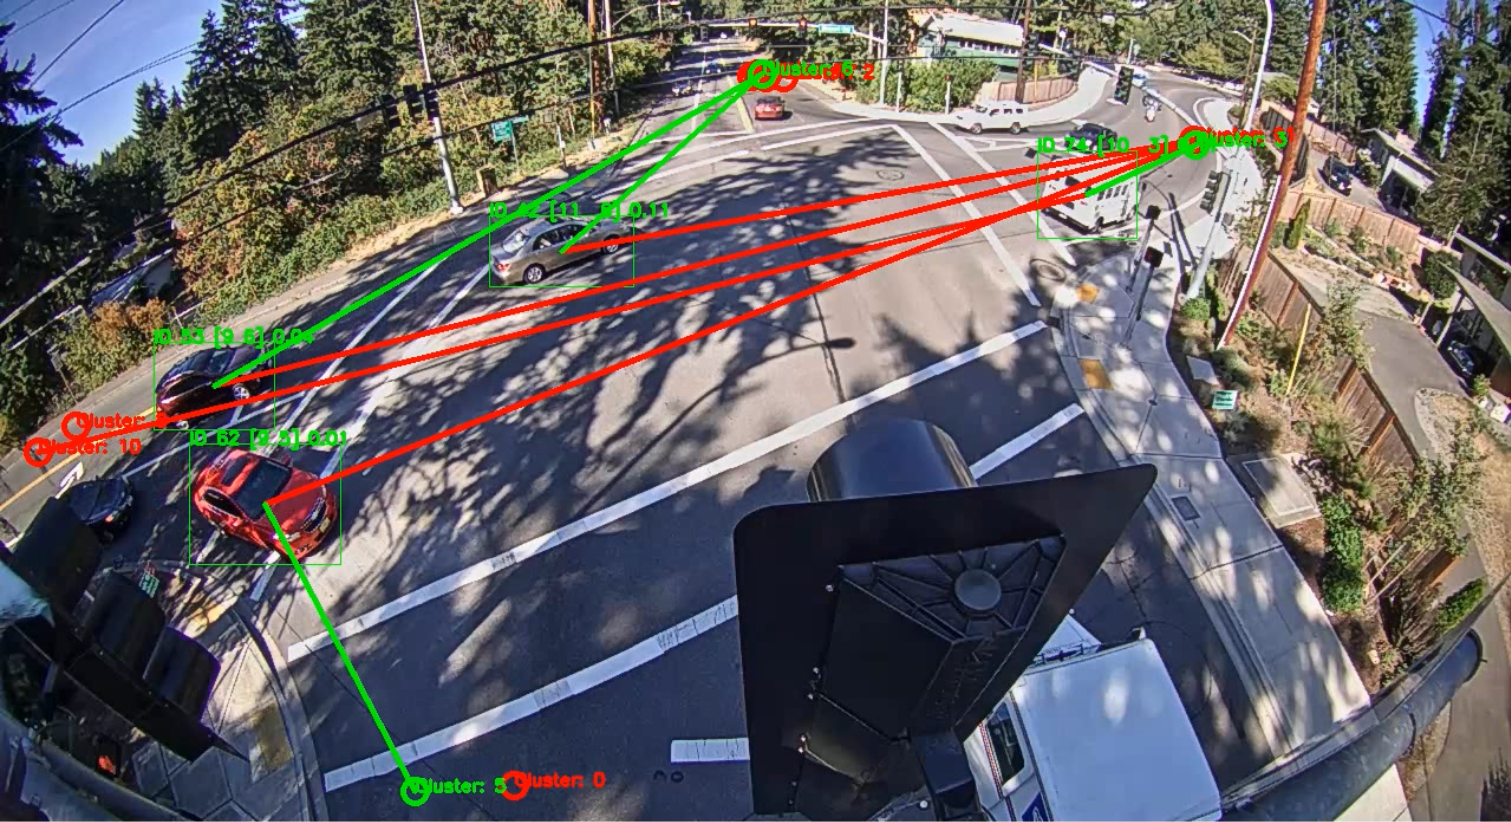
\includegraphics[scale=0.2]{../visualization/bellevue_newport.png}}{Newport_binary_KNN_n_neighbors_15_stride-15_v7.mp4}
\end{frame}



\end{document}